\documentclass[12pt]{article}
\usepackage{amsmath,amsfonts, epsfig}
\usepackage{booktabs} % for better table formatting
\usepackage{array}
\usepackage{multirow}
\usepackage{graphicx}
\usepackage{fancyhdr}
\usepackage{bm}
\pagestyle{fancy}
\lfoot{\texttt{ematm0067.github.io}}
\lhead{Introduction to AI - 03.3\_training - Conor}
\rhead{\thepage}
\cfoot{}

\usepackage{tikz}
\usetikzlibrary{positioning}

\usetikzlibrary{shapes.misc}


\usepackage{ifthen,calc}
\newboolean{nopics}
\setboolean{nopics}{false}


\begin{document}

\section*{Training a neural network.} 

In the last section we looked at how neural networks are able to
perform difficult inference tasks: through the careful choice of
weights and biases they can produce complicated non-linear
functions. This does not explain their power, there are lots of ways
to produce complicated function, the challenge is learning the
functions from data and we haven't discussed how neural networks are
trained. We will discuss that here, but in a way that won't explain
the full power of these networks; there is an unreasonable
effectiveness to learning in deep-learning neural networks, deep here
many networks with many layers and the role deepness plays in this
unreasonable effectiveness is one of the mysteries.

Sometimes too much is made of the fact that we don't fully understand
how deep learning networks work, or, rather, why they work so
well. However, one of the glories of engineering is that something can
be useful even if you don't fully understand it and a mystery, of
course, is exciting for scientists, it is a door you can hope to pass
through.

Anyway, we have already touched on the mechanism used to train a
neural network. Basically, if you have an objective function, a
measure how well something is working and some parameters that adjust
the performance of the network as quantified using the objective
function, then you can use some hill-climbing or optimisation
algorithm to improve the performance and, in the case of neural
networks, that algorithm is a variant of stochastic gradient
descent\footnote{Here, as in a number of places in mathematics, we are
very sloppy about which way we think of as up! We talk about
hill-climbing algorithms and stochastic gradient descent, even though
descending means going down, not climbing. This happens because, of
course, the notion of up and down is metaphorical, are we minimising
an error function or maximising some sort of likelihood function?
Usually, by convention these days we head downwards, so if we are
using a likelihood function we add a minus, but it is just a
convention and all our terminology hasn't quite caught up. The other
place you'll often see and up versus down confusion is when talking
about search trees where you usually imagine the tree with the roots
at the top!}. We have already seen the essential ingredients for this
when we looked at logistic regression; basically we use cross-entropy
loss as the objective and optimize it.

\section*{Cross-entropy loss and SGD}

Lets consider a typical situation, you have input $\mathbf{x}$ and
output $\mathbf{y}$ so that $\mathbf{y}(\textbf{x};\theta)$ and the
$\theta$ are a set of parameters. In the most straight-forward case
these parameters will weights and biases for a neural
network. Typically there will be a dataset
\begin{equation}
  \mathcal{D}=\{(\mathbf{x}^a,\mathbf{y}^a)|a=1\ldots N\}
\end{equation}
so, here, there are $N$ data points and I am using a superscript as
the data index, a subscript will be used for the components of the
vector, so the first data point in the list is
\begin{equation}
  \mathbf{x}^1=(x^1_1,x^1_2,\ldots,x^1_{n_x})
\end{equation}
and $n_x$ here is the size of the input, we will use $n_y$ for the
size of the output. For a classification problem the $\mathbf{y}^a$
will be \textsl{one hot vectors}, which means they will have a single
one value corresponding to the class of the item and zeros for all the
other entries, so if the first item in the data set belongs to class
$k$ then
\begin{equation}
  \mathbf{y}^1=(0,0,\ldots,1,\ldots,0,0)
\end{equation}
Now we are using notation that is potentially confusing, $\mathbf{y}$
without a superscript is a function, so $\mathbf{y}(\mathbf{x}^a)$ is
a set of numbers calculated using the neural network based on the
input $\mathbf{x}^a$.

We are ready to define the cross entropy loss, it is
\begin{equation}
  \mathcal{L}=-\frac{1}{N}\sum_{a=1}^N \sum_{i=1}^{n_y}y_i^a \log{p_i^a}
\end{equation}
where
\begin{equation}
  p_i^a=\sigma_i(\mathbf{y}^a)
\end{equation}
is the softmax. The second sum in the loss function has only one term
since $y_i^a$ is mostly zero:
\begin{equation}
  -\sum_{i=1}^{n_y}y_i^a \log{p_i^a}=-\log{p_k^a}
\end{equation}
if the $a$th item belongs to class $k$. We can see that minimizing
this is good, we want this probability to be close to one and
$\log{1}=0$ while the log of numbers less than one are negative. 

The standard way to minimize this is some version of gradient flow. We
discussed gradient flow before when looking at regression; the idea is
that we change all the parameters by a small amount along a direction
that points down the $L$ landscape:
\begin{equation}
  \theta\leftarrow\theta-\eta\frac{\partial \mathcal{L}}{\partial \theta}
\end{equation}
where $\theta$ is a parameter of the model, one of the $W$s or $b$s,
$\eta$ is the learning rate, a small number which allows the algorithm
to move down towards the minimum, hopefully fast enough not to take
forever, but with steps small enough not to overshoot and cause
unstable, oscillating behaviour. Now the problem is how to calculate
all the derivatives.

At first this looks like it would be impossibly difficult, the models
are very complicated and so calculating all the derivatives would be a
lot of work. It is a lot of work, but we do not have to do it, the
computer does it for us. This is one of the unsung miracles of our
current age, basically, using the chain rule we know how to
differentiate functions that can be written as one thing after
another: if $y(x)=f(g(x))$, so you get $u$ from $x$ first by doing $g$
to it and then $f$ to the result, we know that the rate of change of
$y$ with $x$ is the multiple of how much $f$ changes with $g$ by how
much $g$ changes with $x$:
\begin{equation}
  \frac{dy}{dx}=\frac{df}{dg}\frac{dg}{dx}
\end{equation}
Now, when we programme the neural network we are essentially telling
the computer how do the calculation step-by-step, ultimately to
calculate the computer breaks these instructions into still smaller
steps, a series of elementary operations. The programme can keep track
of these elementary steps and use the chain rule, and the product
rule, to work out the derivative, this is called \texttt{autograd} and
is an essential component of what has made modern machine learning
possible, until recently, the human did the calculus, now the machine
does it, allowing us to use much more complicated networks and to
change them without having to redo all the mathematics.

These is another problem; working out $\mathcal{L}$ as defined would
take a long time, for neural networks to work we need to have a lot of
data and so the calculation of the likelihood would take a huge number
of calculations for just one small gradient step. However, it turns
out that using a much smaller subset will give some reasonable sense
of which direction to move in; approximating $\mathcal{L}$ from a
\textsl{batch} of maybe ten or a 100 data points is often enough, the
key thing is to use a different batch for each gradient step until you
have gone through all the data, an achievement often called an
\textsl{epoch}. Hence, we calculate
\begin{equation}
  \mathcal{L}(B)=-\frac{1}{N_B}\sum_{a\in B} \sum_{i=1}^{n_y}y_i^a \log{p_i^a}
\end{equation}
where $B$ is a batch, some $N_B$ sized subset of the total data and then do
\begin{equation}
  \theta\leftarrow\theta-\eta\frac{\partial \mathcal{L}(B)}{\partial \theta}
\end{equation}
for all the parameters $\theta$ before going on to the next batch.


\begin{figure}[htb]
\begin{center}
  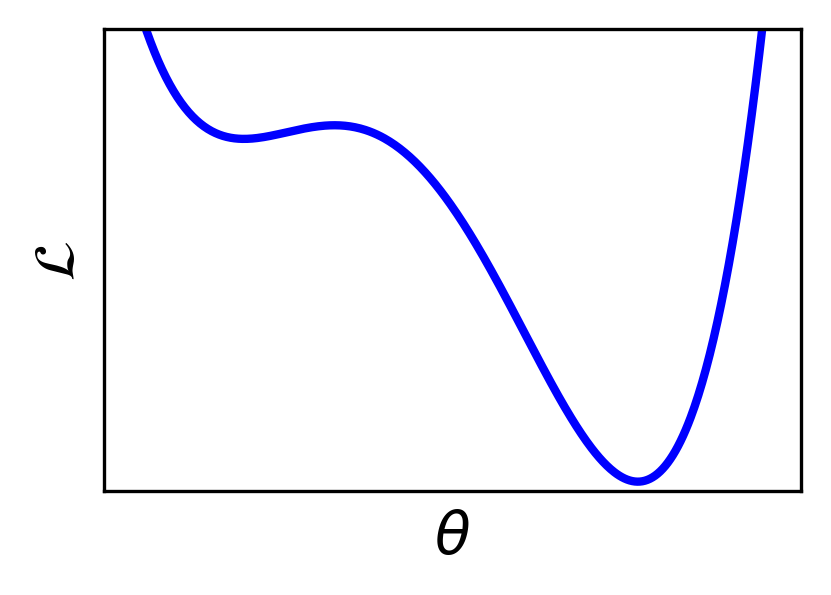
\includegraphics[width=3in]{03.3_objective.png}
\end{center}
\caption{A cartoon of an objective function, the $x$-axis stands in
  for all the many parameter directions. There is a local minimum on
  the left, if the system started off to the left of that and used
  gradient descent it might get stuck in that local minimum. This
  local minimum is intended as a stand-in for the hazards, like thin
  valleys and saddle-points with only a few downward directions that
  might slow down or ruin gradient descent.\label{fig:objective}}
\end{figure}


Weirdly, this process of using batches does not just make optimization
quicker, it also make better. The $\mathcal{L}$ landscape is not a
simple bowl; unlike simpler cases like regression where we expect an
easy optimisation processes, the neural network is designed to produce
non-linear maps and so, inevitably, it has a loss function that may
have local minima and other annoying features: this is sketched out in
Fig.~\ref{fig:objective}. Now if batches are used instead each
gradient step will correspond to a different $\mathcal{L}(B)$ each
approximating the objective, this is illustrated in
Fig.~\ref{fig:objective_noise}. This introduces noise which should
affect some features more than others, meaning that the descent is
less likely to get stuck, the use of batches adds a little randomness
which actually seems to make the optimization more robust.



\begin{figure}[htb]
\begin{center}
  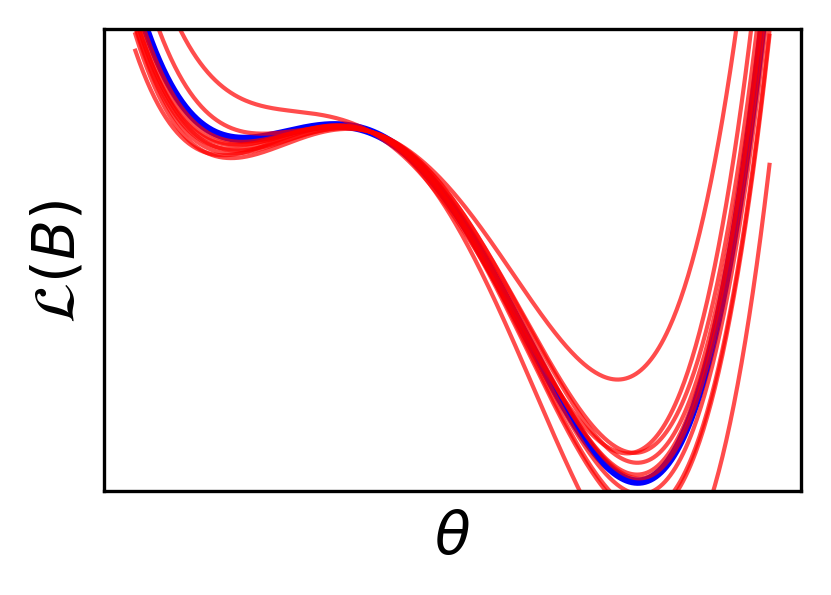
\includegraphics[width=3in]{03.3_objective_noise.png}
\end{center}
\caption{A cartoon of an objective function with batches. Here the blue line represents $\mathcal{L}$ and the red lines $\mathcal{L}(B)$ for different $B$. The local minimum isn't always a minimum and moves around a lot.\label{fig:objective_noise}}
\end{figure}

With this element of randomness this approach is called
\textsl{stochastic gradient descent}, often referred to by its acronym
SGD and is a very standard training algorithm. There are variation we
won't explore further here that try to do things like improve the size
of the gradient step to take into account the local behaviour of
$\mathcal{L}$; the most common of these approaches is probably
\textsl{Adam}. Beyond that there are a huge number of technique for
improving training; for example, in \textsl{dropout} some of the nodes
picked at random are switched off for each training step, this appears
to make training robust and improve behaviour on data points not
included in the training set.





















\end{document}

